\SourceLeaf{266}%
4. In dem rechtwinkligen Dreieck $ABC$ lasse man den Winkel $A$ um $BAB' = dA$
wachsen, während $AB' = c$ bleibt. Fällt man von $B'$ auf $AB$ das Loth $B'C'$, so
entsteht das rechtwinklige Dreieck $AB'C'$ mit den Katheten $a+da$, $b+db$ und der
Hypotenuse $c$; dabei ist $db$ negativ. Macht man auf $B'C'$ $C'D = a$, so wird die
Länge von $BD$:
\[
BD = -g(a) \,.\, db.
\]
Andererseits ist in dem unendlich kleinen Dreieck $BB'D$:
\[
B'D = da
\]
und nach (A):
\[
BB' = f(c) \,.\, dA,
\]
während die Winkel bei $D$ und $B'$ sich nur unendlich wenig von einem Rechten und
$90^{0} - B$ unterscheiden. Mithin ist
\[
BD = \cos B\, f(c) \,.\, dA,
\]
und man hat
\[
\tag*{2)} g(a) \,.\, db = -\cos B\, f(c) \,.\, dA.
\]

\begin{center}\begin{minipage}{\linewidth}\centering
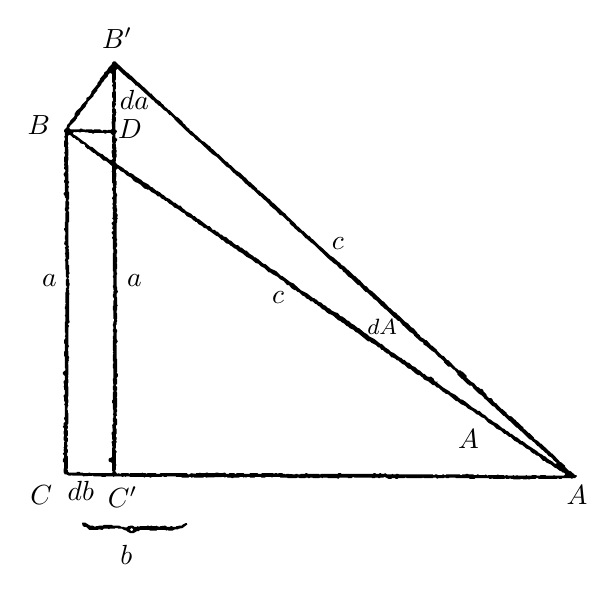
\begin{tikzpicture}[x=0.00782881cm,y=-0.00782881cm]
\fill[even odd rule] (113,825) -- (114,829) -- (116,831) -- (119,831) -- (121,832) -- (125,836) -- (139,836) -- (140,835) -- (146,836) -- (148,834) -- (155,834) -- (157,835) -- (158,834) -- (166,834) -- (167,833) -- (171,833) -- (172,834) -- (178,834) -- (181,836) -- (185,837) -- (187,839) -- (191,841) -- (197,841) -- (202,838) -- (205,838) -- (207,836) -- (222,836) -- (223,837) -- (234,837) -- (235,836) -- (248,836) -- (250,837) -- (252,836) -- (253,837) -- (260,837) -- (264,835) -- (269,835) -- (270,834) -- (276,833) -- (284,827) -- (283,825) -- (281,825) -- (277,827) -- (275,829) -- (270,829) -- (269,830) -- (266,830) -- (265,831) -- (260,831) -- (259,830) -- (257,830) -- (256,831) -- (251,831) -- (248,829) -- (240,830) -- (239,831) -- (235,830) -- (234,829) -- (232,830) -- (227,830) -- (226,829) -- (222,830) -- (221,829) -- (219,829) -- (218,830) -- (207,830) -- (206,831) -- (203,830) -- (202,831) -- (198,831) -- (195,829) -- (191,829) -- (190,830) -- (188,830) -- (186,832) -- (182,832) -- (181,831) -- (177,831) -- (173,829) -- (163,829) -- (162,828) -- (148,828) -- (147,829) -- (140,829) -- (139,830) -- (136,830) -- (134,831) -- (130,829) -- (126,829) -- (118,824) -- (114,824) -- cycle
(193,833) -- (194,833) -- (196,835) -- (196,836) -- (194,838) -- (193,838) -- (191,836) -- (191,835) -- cycle
(162,78) -- (161,81) -- (156,86) -- (153,91) -- (149,94) -- (149,96) -- (142,104) -- (142,106) -- (138,111) -- (138,113) -- (128,125) -- (128,127) -- (126,131) -- (124,133) -- (120,135) -- (120,139) -- (113,146) -- (110,151) -- (104,156) -- (101,161) -- (101,164) -- (100,166) -- (94,172) -- (92,176) -- (89,179) -- (88,183) -- (84,187) -- (84,190) -- (85,191) -- (85,197) -- (84,198) -- (85,200) -- (85,204) -- (84,205) -- (84,214) -- (85,215) -- (85,223) -- (84,224) -- (85,226) -- (85,230) -- (84,231) -- (84,239) -- (85,241) -- (84,242) -- (84,244) -- (85,246) -- (84,247) -- (84,250) -- (86,252) -- (86,254) -- (83,259) -- (85,263) -- (85,268) -- (84,269) -- (84,272) -- (85,273) -- (85,285) -- (86,287) -- (83,290) -- (83,291) -- (85,294) -- (85,296) -- (87,298) -- (87,302) -- (86,303) -- (86,313) -- (85,314) -- (85,317) -- (87,320) -- (86,322) -- (86,336) -- (85,337) -- (85,343) -- (86,345) -- (84,347) -- (84,349) -- (86,353) -- (86,358) -- (85,359) -- (85,364) -- (86,365) -- (86,367) -- (85,368) -- (84,372) -- (87,375) -- (87,376) -- (85,378) -- (86,380) -- (86,386) -- (85,388) -- (86,389) -- (86,393) -- (87,394) -- (85,399) -- (86,400) -- (86,413) -- (87,414) -- (87,425) -- (88,426) -- (88,429) -- (87,430) -- (87,439) -- (88,440) -- (88,443) -- (87,444) -- (87,450) -- (86,451) -- (86,467) -- (87,469) -- (86,470) -- (86,473) -- (85,474) -- (85,477) -- (86,478) -- (86,487) -- (85,488) -- (86,490) -- (86,498) -- (85,499) -- (85,515) -- (86,516) -- (86,520) -- (85,522) -- (86,523) -- (86,525) -- (84,528) -- (84,533) -- (85,534) -- (85,546) -- (84,547) -- (84,554) -- (85,555) -- (85,573) -- (86,574) -- (86,577) -- (82,580) -- (82,583) -- (85,586) -- (85,593) -- (83,595) -- (83,598) -- (84,599) -- (84,602) -- (83,604) -- (84,605) -- (84,608) -- (85,609) -- (85,616) -- (83,618) -- (83,620) -- (84,621) -- (84,627) -- (85,628) -- (85,631) -- (84,632) -- (85,634) -- (85,653) -- (84,654) -- (84,656) -- (86,660) -- (83,663) -- (83,667) -- (82,668) -- (82,669) -- (84,671) -- (84,675) -- (83,676) -- (83,680) -- (84,681) -- (84,684) -- (83,685) -- (83,690) -- (85,692) -- (84,694) -- (84,701) -- (83,702) -- (84,704) -- (83,706) -- (84,710) -- (82,712) -- (82,713) -- (84,715) -- (84,718) -- (82,722) -- (82,725) -- (84,727) -- (84,736) -- (83,737) -- (83,742) -- (85,746) -- (88,746) -- (92,748) -- (95,748) -- (96,747) -- (98,748) -- (114,748) -- (115,749) -- (131,748) -- (132,749) -- (144,749) -- (145,750) -- (151,750) -- (152,749) -- (163,749) -- (164,750) -- (166,749) -- (177,749) -- (178,750) -- (182,749) -- (184,750) -- (185,749) -- (190,749) -- (191,750) -- (213,750) -- (214,751) -- (216,750) -- (222,750) -- (223,751) -- (225,751) -- (226,750) -- (242,750) -- (243,749) -- (245,749) -- (246,750) -- (250,750) -- (251,749) -- (265,749) -- (266,750) -- (274,750) -- (275,751) -- (286,751) -- (287,750) -- (289,750) -- (290,751) -- (292,751) -- (293,750) -- (295,751) -- (310,751) -- (311,750) -- (313,750) -- (314,751) -- (343,750) -- (345,751) -- (346,750) -- (348,750) -- (349,751) -- (355,751) -- (356,752) -- (358,752) -- (359,751) -- (368,751) -- (369,750) -- (374,750) -- (375,751) -- (377,750) -- (379,751) -- (381,750) -- (385,750) -- (386,751) -- (393,751) -- (394,750) -- (403,750) -- (404,751) -- (410,751) -- (411,750) -- (420,750) -- (421,751) -- (423,750) -- (434,750) -- (435,751) -- (446,751) -- (447,752) -- (461,752) -- (462,751) -- (465,751) -- (466,752) -- (475,752) -- (476,751) -- (479,751) -- (480,752) -- (482,752) -- (483,751) -- (487,751) -- (488,752) -- (498,752) -- (499,751) -- (501,751) -- (503,752) -- (504,751) -- (511,751) -- (512,752) -- (527,752) -- (528,753) -- (529,753) -- (531,751) -- (544,751) -- (545,752) -- (550,752) -- (553,750) -- (555,751) -- (583,751) -- (584,752) -- (588,752) -- (589,751) -- (593,751) -- (594,752) -- (596,752) -- (597,751) -- (602,751) -- (604,750) -- (610,753) -- (615,753) -- (616,752) -- (621,752) -- (622,753) -- (625,753) -- (626,752) -- (636,752) -- (637,751) -- (639,751) -- (640,752) -- (665,752) -- (666,751) -- (668,752) -- (682,752) -- (683,751) -- (687,751) -- (689,753) -- (691,752) -- (700,752) -- (701,751) -- (703,751) -- (704,752) -- (708,752) -- (709,751) -- (719,751) -- (720,752) -- (741,752) -- (742,753) -- (750,753) -- (751,752) -- (773,752) -- (774,753) -- (777,753) -- (778,752) -- (780,753) -- (798,753) -- (800,752) -- (801,753) -- (806,753) -- (808,752) -- (809,753) -- (812,753) -- (813,754) -- (824,754) -- (825,753) -- (828,753) -- (829,754) -- (834,754) -- (835,753) -- (837,754) -- (840,754) -- (841,753) -- (849,753) -- (850,752) -- (853,752) -- (854,753) -- (884,753) -- (885,752) -- (887,753) -- (891,753) -- (892,752) -- (906,752) -- (908,753) -- (909,752) -- (913,752) -- (916,749) -- (915,747) -- (913,747) -- (905,740) -- (903,740) -- (897,734) -- (897,732) -- (890,726) -- (889,726) -- (876,712) -- (875,712) -- (858,696) -- (857,696) -- (853,692) -- (848,689) -- (846,687) -- (846,686) -- (839,679) -- (838,679) -- (832,673) -- (831,673) -- (829,671) -- (829,669) -- (827,668) -- (820,661) -- (819,661) -- (816,657) -- (815,657) -- (810,652) -- (806,651) -- (802,647) -- (802,646) -- (795,640) -- (794,640) -- (787,633) -- (786,631) -- (783,630) -- (780,627) -- (779,624) -- (777,622) -- (773,622) -- (770,619) -- (769,616) -- (764,611) -- (764,609) -- (762,607) -- (759,607) -- (757,605) -- (754,604) -- (749,598) -- (745,596) -- (737,589) -- (737,586) -- (730,579) -- (729,579) -- (727,577) -- (724,577) -- (721,574) -- (720,574) -- (708,561) -- (705,560) -- (700,554) -- (697,553) -- (689,545) -- (689,544) -- (681,537) -- (680,537) -- (672,528) -- (670,528) -- (668,526) -- (664,524) -- (661,521) -- (661,520) -- (657,517) -- (657,516) -- (651,509) -- (647,507) -- (642,501) -- (637,498) -- (627,488) -- (626,488) -- (623,484) -- (619,482) -- (613,476) -- (612,476) -- (602,465) -- (601,465) -- (584,449) -- (579,446) -- (575,441) -- (572,440) -- (563,430) -- (562,430) -- (556,424) -- (555,424) -- (545,414) -- (544,414) -- (538,408) -- (534,406) -- (531,402) -- (530,402) -- (521,394) -- (516,391) -- (500,376) -- (499,376) -- (487,364) -- (486,364) -- (482,359) -- (480,359) -- (472,351) -- (471,351) -- (464,344) -- (463,344) -- (460,341) -- (460,340) -- (444,325) -- (444,324) -- (442,322) -- (441,322) -- (423,305) -- (422,305) -- (417,299) -- (416,299) -- (405,289) -- (404,289) -- (400,285) -- (399,285) -- (397,283) -- (397,282) -- (385,271) -- (384,271) -- (378,264) -- (377,264) -- (370,257) -- (362,252) -- (354,244) -- (353,244) -- (349,239) -- (346,238) -- (334,226) -- (333,226) -- (325,218) -- (324,218) -- (320,213) -- (319,213) -- (311,206) -- (308,205) -- (299,196) -- (298,196) -- (291,189) -- (290,189) -- (287,186) -- (287,185) -- (285,184) -- (281,180) -- (281,179) -- (277,176) -- (275,172) -- (274,172) -- (269,167) -- (265,165) -- (255,155) -- (254,155) -- (250,151) -- (249,151) -- (246,148) -- (246,147) -- (244,145) -- (243,145) -- (240,141) -- (235,138) -- (227,130) -- (226,128) -- (224,128) -- (213,117) -- (212,117) -- (205,110) -- (204,110) -- (193,99) -- (192,99) -- (187,94) -- (186,94) -- (167,76) -- (164,76) -- cycle
(168,252) -- (170,250) -- (172,250) -- (176,254) -- (181,256) -- (186,261) -- (192,264) -- (195,267) -- (195,268) -- (200,272) -- (204,273) -- (206,275) -- (207,275) -- (214,282) -- (218,283) -- (219,284) -- (222,284) -- (226,288) -- (232,291) -- (236,295) -- (239,295) -- (243,299) -- (246,300) -- (248,302) -- (250,302) -- (255,307) -- (259,309) -- (263,313) -- (268,315) -- (276,321) -- (279,322) -- (283,327) -- (290,330) -- (294,334) -- (295,334) -- (297,336) -- (299,336) -- (302,340) -- (308,343) -- (311,346) -- (315,347) -- (319,351) -- (320,351) -- (331,359) -- (334,360) -- (340,366) -- (342,366) -- (347,371) -- (351,372) -- (354,375) -- (355,375) -- (360,379) -- (363,380) -- (367,384) -- (373,387) -- (380,393) -- (388,397) -- (395,403) -- (399,404) -- (403,408) -- (409,411) -- (416,418) -- (418,418) -- (422,421) -- (430,425) -- (434,429) -- (440,432) -- (446,439) -- (449,439) -- (453,444) -- (458,447) -- (460,447) -- (463,450) -- (465,450) -- (471,456) -- (474,457) -- (478,461) -- (481,462) -- (484,465) -- (487,465) -- (491,469) -- (494,470) -- (497,473) -- (498,473) -- (503,478) -- (506,479) -- (511,484) -- (512,484) -- (514,486) -- (516,486) -- (520,488) -- (529,496) -- (532,497) -- (534,499) -- (538,501) -- (542,505) -- (545,506) -- (548,509) -- (553,511) -- (557,515) -- (560,516) -- (577,530) -- (580,530) -- (582,532) -- (590,536) -- (594,540) -- (596,540) -- (599,544) -- (601,544) -- (605,548) -- (606,548) -- (608,550) -- (610,550) -- (615,556) -- (617,556) -- (621,558) -- (624,561) -- (626,561) -- (633,567) -- (636,568) -- (642,574) -- (646,575) -- (655,583) -- (659,585) -- (661,585) -- (664,588) -- (665,588) -- (668,592) -- (675,595) -- (682,601) -- (685,601) -- (689,605) -- (691,605) -- (700,613) -- (701,613) -- (703,615) -- (707,616) -- (720,627) -- (722,627) -- (728,632) -- (735,635) -- (739,639) -- (747,643) -- (754,649) -- (756,649) -- (761,653) -- (766,655) -- (772,662) -- (781,667) -- (786,672) -- (793,675) -- (798,680) -- (800,680) -- (806,685) -- (808,685) -- (814,691) -- (820,694) -- (823,697) -- (827,698) -- (834,704) -- (839,706) -- (841,708) -- (841,709) -- (845,712) -- (847,712) -- (850,715) -- (854,716) -- (861,724) -- (864,724) -- (867,727) -- (874,730) -- (880,735) -- (883,736) -- (888,740) -- (891,741) -- (893,743) -- (895,743) -- (897,745) -- (897,746) -- (895,748) -- (880,748) -- (879,747) -- (877,748) -- (866,748) -- (865,747) -- (857,747) -- (856,748) -- (851,748) -- (850,747) -- (843,747) -- (842,748) -- (835,748) -- (834,747) -- (832,748) -- (820,748) -- (819,747) -- (817,748) -- (814,748) -- (813,747) -- (811,748) -- (804,748) -- (803,747) -- (801,747) -- (800,748) -- (798,748) -- (797,747) -- (789,747) -- (788,746) -- (786,747) -- (772,747) -- (771,748) -- (768,746) -- (767,747) -- (757,747) -- (756,746) -- (754,746) -- (753,747) -- (749,747) -- (748,746) -- (740,746) -- (739,745) -- (736,745) -- (735,746) -- (730,746) -- (729,747) -- (727,747) -- (726,746) -- (704,746) -- (703,747) -- (701,747) -- (700,746) -- (698,746) -- (697,747) -- (690,747) -- (689,746) -- (686,746) -- (685,747) -- (683,747) -- (682,746) -- (627,746) -- (626,745) -- (623,745) -- (622,746) -- (618,746) -- (617,745) -- (615,746) -- (608,746) -- (605,744) -- (603,745) -- (599,745) -- (598,744) -- (596,744) -- (595,745) -- (590,745) -- (589,744) -- (586,744) -- (585,745) -- (534,745) -- (533,744) -- (529,744) -- (528,745) -- (501,745) -- (500,746) -- (498,746) -- (497,745) -- (479,745) -- (478,744) -- (476,744) -- (475,745) -- (468,745) -- (467,746) -- (463,746) -- (462,745) -- (460,745) -- (459,746) -- (445,745) -- (443,746) -- (442,745) -- (439,745) -- (438,744) -- (432,744) -- (431,745) -- (429,744) -- (426,744) -- (425,745) -- (423,744) -- (405,744) -- (404,745) -- (399,745) -- (398,744) -- (386,744) -- (385,745) -- (376,745) -- (375,744) -- (364,744) -- (363,745) -- (361,745) -- (360,744) -- (352,744) -- (351,745) -- (347,745) -- (345,743) -- (343,743) -- (342,744) -- (335,744) -- (334,743) -- (330,743) -- (329,744) -- (318,744) -- (317,743) -- (314,743) -- (313,744) -- (306,744) -- (304,743) -- (303,744) -- (298,744) -- (297,745) -- (290,744) -- (287,746) -- (285,746) -- (283,744) -- (240,744) -- (239,745) -- (234,745) -- (233,744) -- (219,744) -- (217,745) -- (216,744) -- (212,744) -- (211,743) -- (209,744) -- (191,744) -- (190,745) -- (188,744) -- (177,744) -- (176,745) -- (172,744) -- (170,745) -- (167,741) -- (167,739) -- (168,738) -- (168,732) -- (169,731) -- (168,729) -- (168,711) -- (169,710) -- (169,708) -- (167,706) -- (167,704) -- (168,703) -- (168,695) -- (169,694) -- (169,692) -- (168,691) -- (169,689) -- (169,686) -- (168,685) -- (168,681) -- (169,680) -- (169,672) -- (168,671) -- (168,667) -- (170,665) -- (170,657) -- (168,654) -- (168,652) -- (170,650) -- (169,648) -- (169,645) -- (170,644) -- (170,641) -- (169,640) -- (169,638) -- (170,637) -- (170,622) -- (169,621) -- (170,619) -- (170,613) -- (169,612) -- (169,610) -- (170,609) -- (170,604) -- (168,602) -- (168,601) -- (170,599) -- (170,592) -- (169,590) -- (171,587) -- (171,583) -- (169,581) -- (170,579) -- (170,559) -- (169,558) -- (169,536) -- (168,535) -- (171,530) -- (169,526) -- (169,516) -- (170,515) -- (170,512) -- (168,509) -- (168,504) -- (169,503) -- (169,499) -- (170,498) -- (170,496) -- (169,495) -- (170,493) -- (170,485) -- (169,484) -- (169,480) -- (170,479) -- (170,473) -- (171,472) -- (170,470) -- (170,459) -- (169,458) -- (169,453) -- (171,450) -- (171,448) -- (170,447) -- (170,442) -- (169,441) -- (169,422) -- (170,421) -- (170,419) -- (169,418) -- (169,413) -- (170,412) -- (170,404) -- (169,403) -- (170,401) -- (170,394) -- (169,393) -- (169,388) -- (170,387) -- (170,382) -- (168,379) -- (170,375) -- (170,371) -- (169,370) -- (169,367) -- (170,366) -- (170,364) -- (169,363) -- (169,338) -- (170,337) -- (170,332) -- (171,331) -- (170,329) -- (171,325) -- (169,322) -- (169,320) -- (170,319) -- (170,315) -- (169,314) -- (169,309) -- (168,308) -- (169,306) -- (169,295) -- (170,294) -- (170,292) -- (168,288) -- (168,281) -- (169,280) -- (168,278) -- (169,276) -- (169,270) -- (168,269) -- (169,258) -- (168,257) -- cycle
(92,195) -- (95,196) -- (99,200) -- (101,200) -- (104,203) -- (107,204) -- (111,209) -- (116,210) -- (118,212) -- (118,214) -- (122,218) -- (124,218) -- (131,224) -- (134,225) -- (138,229) -- (141,230) -- (148,237) -- (151,237) -- (153,238) -- (162,246) -- (162,253) -- (161,254) -- (162,256) -- (162,273) -- (163,274) -- (163,277) -- (164,278) -- (162,282) -- (162,285) -- (163,286) -- (163,291) -- (164,292) -- (163,296) -- (162,297) -- (162,299) -- (163,300) -- (163,306) -- (162,307) -- (163,309) -- (163,312) -- (162,314) -- (163,315) -- (163,318) -- (164,319) -- (163,321) -- (163,329) -- (162,331) -- (164,333) -- (164,335) -- (161,338) -- (161,339) -- (163,342) -- (162,347) -- (164,349) -- (164,350) -- (161,353) -- (161,354) -- (163,357) -- (163,360) -- (162,361) -- (162,363) -- (163,364) -- (163,380) -- (164,381) -- (164,386) -- (163,387) -- (163,416) -- (164,417) -- (164,423) -- (163,424) -- (163,426) -- (164,427) -- (164,439) -- (163,440) -- (163,442) -- (164,443) -- (164,446) -- (165,447) -- (164,449) -- (164,453) -- (163,454) -- (163,457) -- (165,461) -- (165,463) -- (164,464) -- (164,472) -- (163,473) -- (163,479) -- (164,480) -- (164,493) -- (165,494) -- (165,497) -- (164,498) -- (164,501) -- (163,502) -- (163,505) -- (164,506) -- (164,510) -- (163,511) -- (163,514) -- (164,515) -- (164,521) -- (163,522) -- (163,526) -- (164,527) -- (163,529) -- (163,545) -- (164,546) -- (163,548) -- (164,550) -- (163,552) -- (163,562) -- (164,563) -- (164,566) -- (163,567) -- (163,573) -- (164,574) -- (164,590) -- (163,591) -- (164,602) -- (163,603) -- (163,608) -- (164,609) -- (164,612) -- (163,613) -- (163,625) -- (162,626) -- (162,630) -- (163,631) -- (163,640) -- (164,641) -- (164,647) -- (163,648) -- (164,650) -- (164,654) -- (163,655) -- (163,660) -- (164,661) -- (164,663) -- (162,666) -- (163,676) -- (161,678) -- (161,681) -- (162,682) -- (162,689) -- (163,690) -- (163,691) -- (161,693) -- (161,695) -- (162,696) -- (162,700) -- (163,701) -- (162,703) -- (162,717) -- (160,719) -- (158,719) -- (156,721) -- (156,724) -- (158,726) -- (160,726) -- (162,728) -- (162,740) -- (163,742) -- (161,744) -- (127,744) -- (126,743) -- (124,743) -- (123,744) -- (115,744) -- (114,743) -- (110,743) -- (109,742) -- (105,742) -- (104,743) -- (92,743) -- (90,741) -- (90,739) -- (89,738) -- (90,736) -- (90,717) -- (89,716) -- (89,711) -- (90,710) -- (90,706) -- (89,705) -- (89,701) -- (90,700) -- (89,698) -- (89,693) -- (90,692) -- (90,687) -- (89,686) -- (89,684) -- (90,683) -- (90,675) -- (89,674) -- (89,672) -- (90,671) -- (90,668) -- (89,666) -- (91,663) -- (91,647) -- (90,646) -- (90,642) -- (89,641) -- (90,635) -- (91,634) -- (90,632) -- (90,630) -- (91,629) -- (91,625) -- (90,624) -- (90,620) -- (91,619) -- (91,604) -- (90,603) -- (90,598) -- (91,597) -- (91,592) -- (90,591) -- (90,589) -- (91,588) -- (90,586) -- (91,584) -- (91,568) -- (90,566) -- (91,565) -- (91,562) -- (92,561) -- (91,559) -- (92,557) -- (92,555) -- (91,554) -- (91,546) -- (90,545) -- (91,539) -- (92,538) -- (91,536) -- (91,507) -- (92,505) -- (90,502) -- (93,499) -- (93,497) -- (92,496) -- (92,455) -- (93,453) -- (92,452) -- (92,447) -- (91,446) -- (92,444) -- (92,440) -- (93,439) -- (93,436) -- (92,435) -- (92,430) -- (91,429) -- (91,427) -- (92,426) -- (91,422) -- (93,420) -- (93,419) -- (92,418) -- (92,407) -- (91,406) -- (91,400) -- (90,399) -- (90,398) -- (92,396) -- (92,385) -- (91,384) -- (92,382) -- (91,380) -- (91,378) -- (92,377) -- (91,375) -- (91,337) -- (92,336) -- (92,320) -- (91,319) -- (91,316) -- (92,315) -- (92,312) -- (91,311) -- (92,309) -- (92,304) -- (91,303) -- (91,300) -- (92,299) -- (92,288) -- (91,287) -- (91,281) -- (92,279) -- (91,278) -- (91,274) -- (92,273) -- (92,271) -- (91,270) -- (91,258) -- (90,257) -- (91,255) -- (91,245) -- (90,244) -- (90,237) -- (91,236) -- (91,231) -- (90,230) -- (91,228) -- (91,219) -- (90,218) -- (91,216) -- (90,214) -- (90,211) -- (91,210) -- (91,208) -- (90,207) -- (90,197) -- cycle
(98,192) -- (100,190) -- (102,190) -- (103,191) -- (105,190) -- (107,190) -- (108,191) -- (111,191) -- (112,190) -- (117,190) -- (118,191) -- (123,191) -- (124,192) -- (129,192) -- (130,193) -- (132,193) -- (133,192) -- (149,192) -- (150,193) -- (152,193) -- (153,192) -- (159,192) -- (163,196) -- (162,198) -- (162,207) -- (163,208) -- (162,210) -- (162,217) -- (163,219) -- (161,221) -- (161,225) -- (162,226) -- (162,231) -- (163,232) -- (163,234) -- (161,236) -- (157,235) -- (154,232) -- (150,230) -- (146,226) -- (144,226) -- (139,223) -- (130,215) -- (126,214) -- (118,207) -- (117,207) -- (104,197) -- (100,195) -- (98,193) -- cycle
(160,95) -- (162,97) -- (162,110) -- (163,111) -- (163,113) -- (162,114) -- (162,116) -- (163,117) -- (163,125) -- (162,126) -- (162,134) -- (163,135) -- (163,140) -- (162,141) -- (162,150) -- (163,152) -- (162,153) -- (162,159) -- (163,161) -- (162,162) -- (162,169) -- (161,170) -- (162,172) -- (161,174) -- (162,185) -- (160,187) -- (155,187) -- (154,188) -- (152,187) -- (148,187) -- (147,188) -- (145,188) -- (142,186) -- (133,186) -- (132,187) -- (130,187) -- (129,186) -- (120,186) -- (118,187) -- (117,186) -- (114,186) -- (113,185) -- (110,185) -- (109,186) -- (94,186) -- (92,184) -- (94,180) -- (103,171) -- (103,170) -- (105,168) -- (105,166) -- (110,161) -- (110,159) -- (119,149) -- (120,146) -- (122,144) -- (122,142) -- (132,132) -- (132,130) -- (138,123) -- (138,121) -- (144,114) -- (145,111) -- (149,107) -- (149,106) -- (155,100) -- (155,98) -- (158,95) -- cycle
(168,90) -- (170,88) -- (171,88) -- (181,98) -- (182,98) -- (188,104) -- (193,107) -- (199,113) -- (200,115) -- (202,115) -- (228,139) -- (229,139) -- (233,144) -- (234,144) -- (238,148) -- (239,148) -- (246,155) -- (250,157) -- (255,163) -- (257,163) -- (263,169) -- (263,170) -- (289,195) -- (294,198) -- (298,203) -- (299,203) -- (303,207) -- (304,207) -- (324,226) -- (332,231) -- (339,238) -- (340,240) -- (341,240) -- (348,247) -- (352,249) -- (359,257) -- (360,257) -- (365,262) -- (366,262) -- (370,266) -- (371,266) -- (379,275) -- (380,275) -- (385,280) -- (386,280) -- (390,284) -- (391,284) -- (401,294) -- (402,294) -- (409,301) -- (410,301) -- (417,308) -- (417,309) -- (425,316) -- (426,316) -- (434,325) -- (438,326) -- (447,335) -- (448,335) -- (450,337) -- (450,339) -- (454,343) -- (455,343) -- (459,348) -- (460,348) -- (465,353) -- (468,354) -- (476,363) -- (477,363) -- (486,371) -- (487,371) -- (516,399) -- (517,399) -- (521,403) -- (526,406) -- (531,412) -- (534,413) -- (536,415) -- (536,416) -- (538,418) -- (539,418) -- (545,425) -- (550,428) -- (561,439) -- (563,439) -- (573,450) -- (575,450) -- (582,457) -- (583,457) -- (586,461) -- (591,464) -- (599,473) -- (600,473) -- (605,478) -- (606,478) -- (620,492) -- (621,492) -- (626,497) -- (628,497) -- (634,505) -- (635,505) -- (645,515) -- (649,517) -- (652,520) -- (652,521) -- (662,530) -- (665,531) -- (667,533) -- (667,535) -- (672,538) -- (680,545) -- (685,548) -- (692,556) -- (693,556) -- (700,562) -- (700,564) -- (707,571) -- (711,571) -- (716,576) -- (717,576) -- (722,582) -- (722,584) -- (729,591) -- (730,591) -- (739,600) -- (740,600) -- (742,602) -- (745,602) -- (747,604) -- (747,605) -- (757,615) -- (762,618) -- (765,621) -- (765,622) -- (767,624) -- (768,624) -- (779,635) -- (782,636) -- (787,642) -- (788,642) -- (797,651) -- (798,651) -- (806,659) -- (807,659) -- (818,670) -- (819,670) -- (825,676) -- (826,676) -- (839,689) -- (842,690) -- (845,693) -- (846,693) -- (852,700) -- (853,700) -- (859,706) -- (860,706) -- (865,711) -- (866,711) -- (870,716) -- (874,718) -- (877,721) -- (877,722) -- (883,727) -- (883,728) -- (882,729) -- (879,728) -- (876,725) -- (869,721) -- (865,717) -- (862,716) -- (860,714) -- (854,711) -- (851,708) -- (834,697) -- (831,694) -- (830,694) -- (828,692) -- (826,692) -- (819,686) -- (816,685) -- (810,680) -- (808,680) -- (804,676) -- (801,675) -- (798,672) -- (795,671) -- (787,664) -- (781,661) -- (776,657) -- (773,656) -- (767,650) -- (763,648) -- (758,643) -- (755,643) -- (753,641) -- (746,637) -- (734,627) -- (733,627) -- (731,625) -- (727,624) -- (719,617) -- (711,613) -- (709,611) -- (699,605) -- (689,597) -- (690,595) -- (687,596) -- (684,593) -- (684,591) -- (679,587) -- (677,588) -- (673,587) -- (669,583) -- (667,583) -- (662,578) -- (658,576) -- (654,572) -- (649,570) -- (644,565) -- (640,564) -- (636,560) -- (634,560) -- (631,557) -- (628,556) -- (619,549) -- (614,547) -- (610,543) -- (605,540) -- (599,534) -- (597,534) -- (587,526) -- (579,522) -- (575,518) -- (571,516) -- (563,509) -- (560,508) -- (554,503) -- (550,501) -- (546,497) -- (543,496) -- (539,492) -- (538,492) -- (536,490) -- (532,489) -- (528,484) -- (524,483) -- (518,480) -- (515,477) -- (512,476) -- (508,472) -- (505,471) -- (501,467) -- (497,466) -- (493,462) -- (492,462) -- (490,460) -- (488,460) -- (478,452) -- (468,447) -- (456,436) -- (451,434) -- (438,424) -- (436,424) -- (428,416) -- (419,412) -- (411,405) -- (407,404) -- (398,396) -- (397,396) -- (395,394) -- (393,394) -- (390,391) -- (385,388) -- (380,383) -- (378,383) -- (372,378) -- (370,378) -- (366,374) -- (363,374) -- (361,372) -- (360,372) -- (355,367) -- (352,366) -- (347,361) -- (343,360) -- (340,357) -- (338,357) -- (333,352) -- (331,352) -- (328,349) -- (325,349) -- (320,343) -- (317,343) -- (303,332) -- (300,331) -- (296,327) -- (294,327) -- (290,323) -- (282,319) -- (278,315) -- (277,315) -- (273,310) -- (270,310) -- (264,305) -- (262,305) -- (255,299) -- (250,297) -- (246,293) -- (242,291) -- (239,288) -- (238,288) -- (236,286) -- (234,286) -- (227,280) -- (225,280) -- (220,275) -- (212,271) -- (209,268) -- (199,262) -- (196,259) -- (192,257) -- (190,257) -- (186,253) -- (183,252) -- (180,249) -- (170,243) -- (167,239) -- (168,237) -- (168,232) -- (169,231) -- (169,226) -- (168,225) -- (169,223) -- (169,220) -- (168,219) -- (169,216) -- (168,215) -- (168,211) -- (167,209) -- (168,208) -- (168,206) -- (170,204) -- (170,201) -- (169,201) -- (167,199) -- (167,194) -- (170,189) -- (167,186) -- (167,174) -- (168,173) -- (168,167) -- (167,166) -- (167,164) -- (168,163) -- (168,160) -- (169,158) -- (168,157) -- (168,154) -- (166,152) -- (166,150) -- (168,146) -- (168,144) -- (167,143) -- (168,141) -- (168,125) -- (167,124) -- (167,121) -- (168,120) -- (168,110) -- (167,109) -- (167,106) -- (168,105) -- cycle;
\node[inner sep=0pt,font=\fontsize{10}{12}\selectfont] at (170,38) {$B'$};
\node[inner sep=0pt,font=\fontsize{10}{12}\selectfont] at (198,139) {$da$};
\node[inner sep=0pt,font=\fontsize{10}{12}\selectfont] at (191,185) {$D$};
\node[inner sep=0pt,font=\fontsize{10}{12}\selectfont] at (43,179) {$B$};
\node[inner sep=0pt,font=\fontsize{10}{12}\selectfont] at (60,432) {$a$};
\node[inner sep=0pt,font=\fontsize{10}{12}\selectfont] at (198,431) {$a$};
\node[inner sep=0pt,font=\fontsize{10}{12}\selectfont] at (528,372) {$c$};
\node[inner sep=0pt,font=\fontsize{10}{12}\selectfont] at (431,459) {$c$};
\node[inner sep=0pt,font=\fontsize{8}{10}\selectfont] at (600,507) {$dA$};
\node[inner sep=0pt,font=\fontsize{10}{12}\selectfont] at (740,689) {$A$};
\node[inner sep=0pt,font=\fontsize{10}{12}\selectfont] at (47,779) {$C$};
\node[inner sep=0pt,font=\fontsize{10}{12}\selectfont] at (111,773) {$db$};
\node[inner sep=0pt,font=\fontsize{10}{12}\selectfont] at (179,783) {$C'$};
\node[inner sep=0pt,font=\fontsize{10}{12}\selectfont] at (185,876) {$b$};
\node[inner sep=0pt,font=\fontsize{10}{12}\selectfont] at (916,779) {$A$};
\end{tikzpicture}


Fig. 5.
\end{minipage}\end{center}

5. Durch Verbindung von 1) und 2) folgt, dass bei dem Übergange von dem Dreieck
$a, b, c; A, B$ zu dem Dreieck $a+da, b+db, c+dc; A+dA, B+dB$ zwischen $db, dc$ und
$dA$ die Relation:
\[
\tag*{I.} g(a) \,.\, db - \sin B \,.\, dc + f(c) \cos B \,.\, dA = 0
\]
besteht. Da man aber gleichzeitig $a$ mit $b$ und $A$ mit $B$ vertauschen darf, so
gilt auch die Gleichung:
\[
\tag*{II.} g(b) \,.\, da - \sin A \,.\, dc + f(c) \cos A \,.\, dB = 0.
\]

\Needspace{34\baselineskip}
6. In dem rechtwinkligen Dreieck $ABC$ lasse man $A$ um $BAB' = dA$ wachsen;
verlängert man $BC$ bis zum Schnitt mit $AB'$, so entsteht das rechtwinklige
Dreieck $ACB'$ mit den Katheten $a+da$ und $b$. Macht man auf $AB'$ $AD = c$, so
wird in dem unendlich kleinen Dreieck $BB'D$:
\[
BB' = da, \qquad BD = f(c) \,.\, dA,
\]
folglich ist
\[
\tag*{3)} f(c) \,.\, dA = \sin B \,.\, da.
\]

\begin{center}\begin{minipage}{\linewidth}\centering
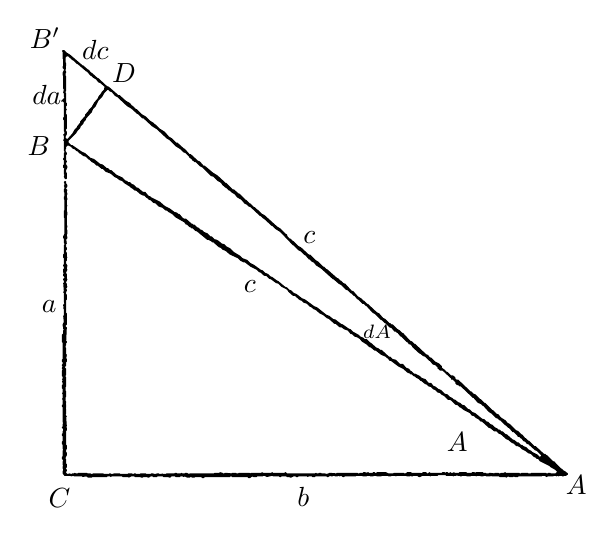
\begin{tikzpicture}[x=0.00771605cm,y=-0.00771605cm]
\fill[even odd rule] (72,57) -- (73,59) -- (73,70) -- (74,71) -- (74,82) -- (73,83) -- (73,85) -- (75,87) -- (75,89) -- (73,93) -- (73,97) -- (74,98) -- (74,119) -- (75,120) -- (74,126) -- (75,127) -- (75,132) -- (76,134) -- (71,139) -- (71,141) -- (73,140) -- (75,142) -- (75,166) -- (74,167) -- (74,170) -- (75,171) -- (75,189) -- (76,190) -- (76,193) -- (74,195) -- (75,197) -- (75,202) -- (74,204) -- (75,205) -- (75,221) -- (76,222) -- (76,224) -- (75,225) -- (75,233) -- (74,234) -- (74,236) -- (75,237) -- (75,244) -- (74,245) -- (74,249) -- (76,251) -- (75,253) -- (75,260) -- (76,261) -- (75,264) -- (77,268) -- (79,268) -- (80,267) -- (80,258) -- (79,257) -- (79,253) -- (81,249) -- (81,247) -- (79,244) -- (79,241) -- (80,240) -- (80,238) -- (79,237) -- (79,228) -- (80,227) -- (80,225) -- (78,222) -- (78,219) -- (79,218) -- (79,215) -- (81,213) -- (83,213) -- (87,215) -- (90,218) -- (93,219) -- (96,222) -- (97,222) -- (101,226) -- (102,226) -- (107,230) -- (111,231) -- (116,236) -- (117,236) -- (121,240) -- (125,242) -- (129,246) -- (131,246) -- (137,251) -- (139,251) -- (144,256) -- (152,259) -- (159,265) -- (162,266) -- (167,270) -- (171,271) -- (175,275) -- (183,280) -- (186,283) -- (187,283) -- (192,287) -- (194,287) -- (201,293) -- (205,295) -- (207,295) -- (211,299) -- (212,299) -- (215,302) -- (218,303) -- (222,307) -- (226,308) -- (231,313) -- (237,315) -- (243,320) -- (245,320) -- (247,322) -- (254,326) -- (259,331) -- (273,339) -- (276,343) -- (278,343) -- (282,347) -- (283,347) -- (285,349) -- (287,349) -- (291,353) -- (294,354) -- (311,368) -- (313,368) -- (317,370) -- (319,372) -- (321,372) -- (330,380) -- (333,381) -- (336,384) -- (341,386) -- (348,392) -- (361,398) -- (365,402) -- (371,405) -- (373,405) -- (382,412) -- (392,417) -- (396,421) -- (399,422) -- (403,426) -- (405,427) -- (408,427) -- (413,432) -- (416,433) -- (424,439) -- (428,440) -- (433,445) -- (441,449) -- (444,452) -- (444,453) -- (452,460) -- (455,460) -- (463,467) -- (466,468) -- (469,471) -- (475,473) -- (480,478) -- (481,478) -- (486,482) -- (489,483) -- (496,489) -- (502,492) -- (508,497) -- (511,498) -- (520,506) -- (522,506) -- (529,512) -- (532,512) -- (536,515) -- (542,517) -- (547,523) -- (549,523) -- (553,527) -- (557,528) -- (562,531) -- (565,535) -- (573,540) -- (577,544) -- (580,545) -- (586,550) -- (588,550) -- (597,557) -- (604,560) -- (607,563) -- (608,563) -- (611,567) -- (613,567) -- (625,576) -- (633,580) -- (641,587) -- (643,587) -- (645,589) -- (647,589) -- (650,592) -- (653,593) -- (655,595) -- (659,597) -- (662,600) -- (663,600) -- (669,605) -- (672,606) -- (675,609) -- (679,610) -- (683,614) -- (686,615) -- (690,619) -- (694,620) -- (697,623) -- (701,625) -- (707,631) -- (710,631) -- (712,632) -- (719,639) -- (723,640) -- (727,644) -- (728,644) -- (733,648) -- (743,653) -- (746,657) -- (750,658) -- (753,661) -- (757,663) -- (761,667) -- (763,667) -- (774,677) -- (777,678) -- (783,683) -- (787,683) -- (791,687) -- (794,688) -- (803,696) -- (806,697) -- (812,702) -- (815,703) -- (819,707) -- (821,707) -- (825,709) -- (828,712) -- (834,715) -- (839,719) -- (843,720) -- (848,725) -- (851,726) -- (853,728) -- (855,728) -- (858,732) -- (874,740) -- (876,742) -- (883,746) -- (886,749) -- (886,750) -- (884,752) -- (876,752) -- (875,751) -- (872,751) -- (871,752) -- (869,752) -- (868,751) -- (844,751) -- (843,752) -- (839,752) -- (838,751) -- (828,751) -- (827,752) -- (825,752) -- (824,751) -- (802,751) -- (801,750) -- (799,751) -- (794,751) -- (793,752) -- (791,752) -- (790,751) -- (784,751) -- (783,752) -- (775,751) -- (774,752) -- (770,752) -- (769,751) -- (765,751) -- (764,750) -- (753,750) -- (752,751) -- (750,750) -- (747,750) -- (746,751) -- (738,751) -- (737,750) -- (726,750) -- (725,751) -- (718,751) -- (717,750) -- (715,751) -- (712,751) -- (711,750) -- (709,751) -- (707,751) -- (706,750) -- (704,750) -- (703,751) -- (701,750) -- (698,750) -- (697,751) -- (678,751) -- (676,750) -- (674,752) -- (673,752) -- (671,750) -- (666,750) -- (663,752) -- (661,751) -- (647,751) -- (646,750) -- (640,750) -- (637,752) -- (635,752) -- (634,751) -- (618,751) -- (617,752) -- (609,752) -- (605,750) -- (590,750) -- (589,751) -- (587,751) -- (586,750) -- (584,750) -- (583,751) -- (577,751) -- (576,750) -- (572,751) -- (571,750) -- (568,750) -- (567,751) -- (562,751) -- (561,752) -- (559,752) -- (558,751) -- (524,751) -- (523,752) -- (512,751) -- (511,752) -- (506,753) -- (505,752) -- (499,752) -- (498,751) -- (495,751) -- (494,752) -- (491,752) -- (490,751) -- (488,752) -- (442,752) -- (440,750) -- (438,751) -- (419,751) -- (418,750) -- (416,751) -- (403,751) -- (401,750) -- (400,751) -- (383,751) -- (382,752) -- (380,751) -- (363,751) -- (362,752) -- (359,752) -- (358,751) -- (352,751) -- (351,752) -- (340,751) -- (339,752) -- (337,752) -- (336,751) -- (332,750) -- (331,751) -- (323,751) -- (322,752) -- (282,752) -- (281,753) -- (277,751) -- (275,751) -- (274,752) -- (270,752) -- (269,751) -- (267,752) -- (261,752) -- (260,751) -- (258,751) -- (257,752) -- (244,752) -- (243,753) -- (238,753) -- (237,752) -- (235,753) -- (232,753) -- (231,752) -- (228,752) -- (227,753) -- (223,753) -- (222,752) -- (219,752) -- (218,753) -- (211,753) -- (210,752) -- (201,752) -- (200,753) -- (194,753) -- (193,752) -- (191,752) -- (190,753) -- (188,753) -- (187,752) -- (181,752) -- (180,753) -- (168,753) -- (167,752) -- (157,752) -- (156,753) -- (153,753) -- (152,752) -- (150,752) -- (149,753) -- (141,753) -- (140,752) -- (123,752) -- (122,753) -- (120,753) -- (119,752) -- (114,752) -- (113,751) -- (99,751) -- (98,752) -- (95,752) -- (93,751) -- (92,752) -- (89,752) -- (88,753) -- (86,753) -- (85,752) -- (81,753) -- (79,751) -- (79,749) -- (80,748) -- (80,746) -- (79,745) -- (79,743) -- (80,742) -- (80,737) -- (79,736) -- (79,729) -- (78,728) -- (78,726) -- (80,722) -- (80,718) -- (79,717) -- (79,713) -- (80,712) -- (80,706) -- (79,705) -- (79,682) -- (80,681) -- (80,677) -- (79,676) -- (80,674) -- (79,660) -- (80,658) -- (78,656) -- (79,654) -- (79,646) -- (78,645) -- (79,643) -- (79,639) -- (78,638) -- (79,636) -- (79,634) -- (78,633) -- (78,627) -- (79,626) -- (79,617) -- (78,616) -- (78,610) -- (79,609) -- (79,594) -- (78,593) -- (78,591) -- (79,590) -- (79,580) -- (77,578) -- (77,577) -- (79,575) -- (79,569) -- (80,568) -- (80,564) -- (79,563) -- (80,557) -- (79,556) -- (79,546) -- (78,545) -- (78,542) -- (79,541) -- (79,538) -- (80,537) -- (80,535) -- (79,534) -- (80,512) -- (78,510) -- (78,509) -- (80,507) -- (80,489) -- (79,488) -- (79,467) -- (80,466) -- (80,458) -- (79,457) -- (79,453) -- (80,452) -- (80,450) -- (79,448) -- (81,445) -- (80,443) -- (80,440) -- (79,439) -- (79,437) -- (81,433) -- (80,431) -- (80,424) -- (79,423) -- (79,421) -- (81,417) -- (80,415) -- (81,410) -- (79,407) -- (79,403) -- (80,402) -- (80,398) -- (81,397) -- (80,395) -- (80,389) -- (79,388) -- (79,385) -- (80,384) -- (80,381) -- (79,380) -- (79,375) -- (80,374) -- (79,367) -- (81,365) -- (81,363) -- (80,362) -- (80,359) -- (81,358) -- (81,352) -- (80,351) -- (80,348) -- (81,347) -- (81,345) -- (80,344) -- (80,328) -- (81,327) -- (81,322) -- (80,321) -- (80,313) -- (81,312) -- (80,310) -- (80,303) -- (81,302) -- (81,299) -- (80,298) -- (80,294) -- (81,293) -- (81,291) -- (80,290) -- (80,288) -- (81,286) -- (79,284) -- (79,283) -- (81,280) -- (81,278) -- (79,275) -- (79,272) -- (77,271) -- (75,273) -- (76,275) -- (76,278) -- (75,279) -- (76,281) -- (76,284) -- (75,285) -- (75,289) -- (76,290) -- (76,296) -- (75,297) -- (75,301) -- (76,302) -- (76,319) -- (75,320) -- (75,331) -- (76,332) -- (76,358) -- (74,362) -- (74,365) -- (75,366) -- (75,373) -- (76,374) -- (76,376) -- (75,377) -- (75,391) -- (74,392) -- (74,397) -- (75,398) -- (75,408) -- (74,409) -- (74,411) -- (75,412) -- (75,415) -- (74,416) -- (74,421) -- (75,423) -- (74,424) -- (74,427) -- (76,429) -- (76,430) -- (74,432) -- (74,434) -- (75,435) -- (75,438) -- (74,439) -- (75,452) -- (74,454) -- (75,455) -- (75,470) -- (76,472) -- (74,475) -- (74,477) -- (75,478) -- (74,480) -- (75,482) -- (75,492) -- (74,493) -- (75,503) -- (73,507) -- (73,510) -- (74,511) -- (74,514) -- (75,516) -- (74,517) -- (74,522) -- (72,524) -- (72,536) -- (73,537) -- (73,564) -- (72,565) -- (72,568) -- (73,569) -- (73,572) -- (72,573) -- (72,575) -- (73,576) -- (72,578) -- (72,580) -- (73,581) -- (72,583) -- (72,592) -- (73,593) -- (73,596) -- (72,597) -- (73,599) -- (72,601) -- (73,603) -- (73,606) -- (72,607) -- (72,612) -- (73,613) -- (73,619) -- (72,620) -- (73,622) -- (73,628) -- (72,630) -- (73,631) -- (73,639) -- (72,640) -- (72,642) -- (73,643) -- (73,668) -- (74,669) -- (73,671) -- (73,675) -- (72,676) -- (72,677) -- (74,679) -- (74,682) -- (73,683) -- (73,686) -- (72,687) -- (72,690) -- (73,691) -- (73,699) -- (72,700) -- (72,704) -- (73,705) -- (73,712) -- (74,713) -- (73,715) -- (73,724) -- (72,725) -- (72,728) -- (74,731) -- (73,733) -- (73,738) -- (74,739) -- (73,741) -- (73,744) -- (74,745) -- (74,747) -- (73,748) -- (73,752) -- (76,756) -- (86,756) -- (87,757) -- (91,756) -- (92,757) -- (105,757) -- (106,758) -- (112,757) -- (115,759) -- (121,759) -- (122,758) -- (146,758) -- (147,757) -- (151,757) -- (152,758) -- (154,757) -- (171,757) -- (172,758) -- (181,758) -- (182,759) -- (186,757) -- (191,757) -- (192,758) -- (201,758) -- (202,759) -- (205,759) -- (206,758) -- (212,758) -- (213,759) -- (215,759) -- (218,757) -- (221,757) -- (222,758) -- (228,758) -- (229,757) -- (238,757) -- (239,758) -- (247,758) -- (248,759) -- (250,759) -- (252,757) -- (258,757) -- (259,758) -- (266,758) -- (267,757) -- (270,757) -- (272,758) -- (274,757) -- (278,759) -- (282,759) -- (283,758) -- (285,758) -- (286,759) -- (290,759) -- (291,758) -- (301,758) -- (303,760) -- (305,760) -- (307,758) -- (348,758) -- (349,757) -- (351,757) -- (352,758) -- (377,758) -- (379,760) -- (381,760) -- (385,757) -- (387,758) -- (392,758) -- (393,757) -- (402,757) -- (403,756) -- (405,756) -- (409,758) -- (418,756) -- (419,757) -- (429,757) -- (430,758) -- (432,758) -- (433,757) -- (441,757) -- (442,758) -- (446,758) -- (447,759) -- (449,759) -- (453,757) -- (456,757) -- (457,758) -- (460,758) -- (461,757) -- (475,757) -- (476,758) -- (478,757) -- (483,757) -- (484,758) -- (488,758) -- (489,757) -- (507,757) -- (508,758) -- (510,758) -- (513,756) -- (515,757) -- (517,757) -- (518,756) -- (520,756) -- (521,757) -- (525,757) -- (527,756) -- (529,757) -- (531,756) -- (534,758) -- (536,758) -- (537,757) -- (555,757) -- (556,756) -- (566,756) -- (567,757) -- (573,757) -- (574,756) -- (578,756) -- (579,757) -- (584,757) -- (585,756) -- (589,756) -- (590,757) -- (597,757) -- (598,756) -- (608,756) -- (609,757) -- (613,757) -- (614,756) -- (620,756) -- (621,757) -- (623,756) -- (638,756) -- (639,757) -- (644,757) -- (646,756) -- (647,757) -- (649,757) -- (650,756) -- (656,756) -- (659,758) -- (661,758) -- (665,756) -- (676,756) -- (678,757) -- (679,756) -- (690,756) -- (691,755) -- (703,755) -- (704,756) -- (714,756) -- (716,757) -- (717,756) -- (720,756) -- (722,755) -- (723,756) -- (726,756) -- (727,757) -- (729,757) -- (730,756) -- (737,756) -- (738,757) -- (744,757) -- (745,756) -- (752,756) -- (753,757) -- (755,756) -- (760,756) -- (761,757) -- (765,757) -- (766,756) -- (769,756) -- (770,757) -- (776,757) -- (778,756) -- (779,757) -- (791,757) -- (792,758) -- (801,758) -- (803,759) -- (806,757) -- (808,758) -- (814,758) -- (815,757) -- (817,758) -- (822,758) -- (823,757) -- (861,757) -- (862,756) -- (866,756) -- (869,758) -- (871,757) -- (880,757) -- (881,756) -- (884,756) -- (885,757) -- (887,756) -- (889,757) -- (891,756) -- (894,756) -- (895,757) -- (897,757) -- (898,756) -- (901,756) -- (904,754) -- (904,752) -- (899,748) -- (898,748) -- (894,744) -- (893,744) -- (884,735) -- (883,733) -- (880,732) -- (870,722) -- (869,722) -- (867,720) -- (865,720) -- (851,707) -- (849,707) -- (840,698) -- (839,698) -- (835,694) -- (834,694) -- (829,688) -- (828,688) -- (822,682) -- (819,681) -- (809,671) -- (805,669) -- (802,665) -- (794,660) -- (790,655) -- (787,654) -- (781,648) -- (780,648) -- (768,636) -- (767,636) -- (761,630) -- (760,630) -- (752,622) -- (749,621) -- (745,617) -- (744,617) -- (724,598) -- (721,598) -- (719,596) -- (719,594) -- (717,592) -- (715,591) -- (712,591) -- (706,585) -- (705,585) -- (700,580) -- (699,580) -- (697,578) -- (697,575) -- (696,575) -- (692,571) -- (686,568) -- (680,562) -- (677,561) -- (674,557) -- (671,556) -- (653,539) -- (652,539) -- (648,535) -- (645,534) -- (633,521) -- (632,521) -- (628,517) -- (623,514) -- (616,507) -- (614,507) -- (612,505) -- (611,505) -- (604,498) -- (600,496) -- (594,489) -- (590,487) -- (575,473) -- (574,473) -- (569,468) -- (568,468) -- (564,464) -- (559,461) -- (551,452) -- (549,452) -- (538,440) -- (535,439) -- (531,435) -- (530,435) -- (526,431) -- (525,431) -- (508,416) -- (507,416) -- (503,412) -- (502,412) -- (494,404) -- (489,401) -- (480,392) -- (478,392) -- (465,380) -- (461,378) -- (453,370) -- (452,370) -- (448,366) -- (447,366) -- (443,362) -- (442,359) -- (440,358) -- (431,349) -- (426,346) -- (405,327) -- (401,325) -- (394,318) -- (393,318) -- (389,314) -- (388,314) -- (382,308) -- (381,308) -- (375,302) -- (374,302) -- (364,292) -- (363,292) -- (355,285) -- (353,285) -- (342,274) -- (341,274) -- (328,262) -- (320,257) -- (307,246) -- (305,246) -- (299,239) -- (296,238) -- (284,227) -- (282,227) -- (274,218) -- (273,218) -- (262,208) -- (260,208) -- (253,201) -- (248,198) -- (241,190) -- (233,185) -- (226,178) -- (225,178) -- (222,175) -- (217,172) -- (210,165) -- (203,161) -- (195,153) -- (194,153) -- (188,147) -- (187,147) -- (184,143) -- (177,139) -- (167,130) -- (165,130) -- (149,116) -- (146,115) -- (132,102) -- (131,102) -- (121,93) -- (120,93) -- (116,88) -- (115,88) -- (107,81) -- (106,81) -- (85,63) -- (80,60) -- (76,56) -- (73,56) -- cycle
(83,205) -- (95,193) -- (98,188) -- (102,184) -- (103,181) -- (107,177) -- (108,174) -- (111,171) -- (112,168) -- (121,158) -- (123,153) -- (127,149) -- (132,139) -- (138,133) -- (142,126) -- (147,121) -- (148,121) -- (151,124) -- (154,125) -- (159,131) -- (163,133) -- (179,148) -- (186,152) -- (196,161) -- (197,161) -- (204,168) -- (206,168) -- (220,181) -- (228,186) -- (244,201) -- (249,204) -- (259,214) -- (267,219) -- (272,224) -- (275,225) -- (281,231) -- (281,232) -- (286,236) -- (287,238) -- (288,238) -- (290,240) -- (292,240) -- (299,247) -- (303,249) -- (317,263) -- (321,264) -- (328,271) -- (332,273) -- (335,276) -- (335,277) -- (342,283) -- (343,283) -- (347,287) -- (348,287) -- (351,290) -- (356,293) -- (360,298) -- (367,302) -- (372,308) -- (376,310) -- (379,313) -- (382,314) -- (398,329) -- (399,329) -- (403,333) -- (404,333) -- (417,345) -- (418,345) -- (423,350) -- (431,355) -- (452,377) -- (453,377) -- (461,385) -- (465,387) -- (471,393) -- (472,393) -- (478,400) -- (479,400) -- (483,404) -- (486,405) -- (490,410) -- (498,415) -- (518,433) -- (519,433) -- (527,440) -- (531,442) -- (539,450) -- (542,451) -- (547,456) -- (548,456) -- (552,460) -- (553,460) -- (558,466) -- (559,466) -- (566,473) -- (568,473) -- (572,477) -- (573,477) -- (583,488) -- (587,490) -- (597,500) -- (598,500) -- (603,505) -- (604,505) -- (611,512) -- (614,513) -- (619,519) -- (621,519) -- (623,521) -- (624,521) -- (629,527) -- (630,527) -- (639,536) -- (640,536) -- (643,540) -- (645,540) -- (648,543) -- (648,544) -- (660,555) -- (661,555) -- (666,559) -- (669,560) -- (676,567) -- (677,567) -- (682,573) -- (686,574) -- (690,578) -- (690,580) -- (691,580) -- (694,583) -- (698,583) -- (712,596) -- (712,598) -- (715,598) -- (719,602) -- (719,604) -- (722,607) -- (724,607) -- (726,609) -- (728,609) -- (748,628) -- (749,628) -- (756,636) -- (761,638) -- (764,641) -- (765,641) -- (774,651) -- (779,654) -- (786,661) -- (789,662) -- (792,665) -- (793,665) -- (801,673) -- (802,673) -- (806,677) -- (807,677) -- (813,684) -- (815,684) -- (821,690) -- (822,692) -- (824,692) -- (827,695) -- (828,695) -- (831,699) -- (834,700) -- (837,704) -- (839,704) -- (850,714) -- (853,715) -- (860,722) -- (860,723) -- (858,725) -- (854,721) -- (846,717) -- (844,715) -- (840,713) -- (836,709) -- (831,707) -- (829,705) -- (827,705) -- (823,701) -- (821,701) -- (816,697) -- (813,696) -- (804,688) -- (801,687) -- (797,683) -- (795,683) -- (792,680) -- (790,680) -- (788,678) -- (784,676) -- (780,672) -- (777,671) -- (773,667) -- (771,667) -- (767,663) -- (763,662) -- (752,653) -- (747,651) -- (743,647) -- (740,646) -- (734,640) -- (730,639) -- (727,636) -- (724,635) -- (719,631) -- (716,630) -- (714,628) -- (710,626) -- (706,622) -- (702,621) -- (696,615) -- (691,613) -- (686,609) -- (683,608) -- (679,603) -- (675,603) -- (670,597) -- (664,595) -- (661,592) -- (653,588) -- (651,588) -- (647,584) -- (646,584) -- (643,580) -- (638,578) -- (633,572) -- (628,572) -- (621,565) -- (616,564) -- (612,560) -- (610,560) -- (598,549) -- (596,549) -- (592,546) -- (589,545) -- (580,537) -- (579,537) -- (573,531) -- (570,531) -- (568,529) -- (563,527) -- (560,524) -- (551,519) -- (547,515) -- (544,514) -- (534,507) -- (531,506) -- (522,499) -- (518,498) -- (512,493) -- (507,491) -- (492,479) -- (487,477) -- (472,466) -- (467,464) -- (458,457) -- (453,455) -- (449,451) -- (446,450) -- (442,446) -- (439,445) -- (427,435) -- (426,435) -- (418,429) -- (415,428) -- (411,424) -- (406,422) -- (402,418) -- (399,417) -- (388,409) -- (382,406) -- (377,401) -- (369,398) -- (365,394) -- (355,388) -- (349,382) -- (343,379) -- (339,375) -- (335,374) -- (329,369) -- (325,367) -- (323,367) -- (318,362) -- (316,362) -- (311,357) -- (306,355) -- (303,352) -- (300,351) -- (297,348) -- (294,347) -- (290,343) -- (288,343) -- (286,341) -- (285,341) -- (276,333) -- (273,333) -- (271,332) -- (265,325) -- (263,325) -- (261,323) -- (257,322) -- (249,316) -- (241,312) -- (233,305) -- (219,298) -- (217,296) -- (215,296) -- (209,289) -- (206,289) -- (204,288) -- (197,282) -- (195,282) -- (190,277) -- (187,276) -- (184,273) -- (181,273) -- (179,271) -- (176,270) -- (171,265) -- (162,261) -- (153,253) -- (151,253) -- (148,250) -- (146,250) -- (139,244) -- (135,243) -- (125,235) -- (119,233) -- (110,225) -- (105,223) -- (89,212) -- (87,212) -- (83,208) -- cycle
(80,66) -- (82,66) -- (90,73) -- (91,73) -- (97,79) -- (98,79) -- (112,91) -- (113,91) -- (119,98) -- (120,98) -- (123,101) -- (128,104) -- (132,109) -- (135,110) -- (142,116) -- (141,121) -- (137,125) -- (137,126) -- (132,132) -- (131,135) -- (125,142) -- (121,149) -- (116,154) -- (116,155) -- (110,162) -- (110,164) -- (102,173) -- (102,175) -- (97,181) -- (97,182) -- (93,186) -- (89,193) -- (81,202) -- (80,202) -- (78,200) -- (78,198) -- (80,194) -- (80,190) -- (79,189) -- (79,186) -- (80,185) -- (80,162) -- (79,161) -- (79,155) -- (80,154) -- (79,152) -- (79,148) -- (80,147) -- (80,143) -- (79,142) -- (79,127) -- (78,126) -- (78,124) -- (79,123) -- (79,99) -- (78,98) -- (78,94) -- (79,93) -- (79,91) -- (78,90) -- (79,77) -- (78,76) -- (78,68) -- cycle;
\node[inner sep=0pt,font=\fontsize{10}{12}\selectfont] at (44,36) {$B'$};
\node[inner sep=0pt,font=\fontsize{10}{12}\selectfont] at (127,56) {$dc$};
\node[inner sep=0pt,font=\fontsize{10}{12}\selectfont] at (47,129) {$da$};
\node[inner sep=0pt,font=\fontsize{10}{12}\selectfont] at (174,93) {$D$};
\node[inner sep=0pt,font=\fontsize{10}{12}\selectfont] at (34,214) {$B$};
\node[inner sep=0pt,font=\fontsize{10}{12}\selectfont] at (51,478) {$a$};
\node[inner sep=0pt,font=\fontsize{10}{12}\selectfont] at (479,364) {$c$};
\node[inner sep=0pt,font=\fontsize{10}{12}\selectfont] at (381,445) {$c$};
\node[inner sep=0pt,font=\fontsize{7}{9}\selectfont] at (590,519) {$dA$};
\node[inner sep=0pt,font=\fontsize{10}{12}\selectfont] at (722,700) {$A$};
\node[inner sep=0pt,font=\fontsize{10}{12}\selectfont] at (68,792) {$C$};
\node[inner sep=0pt,font=\fontsize{10}{12}\selectfont] at (469,791) {$b$};
\node[inner sep=0pt,font=\fontsize{10}{12}\selectfont] at (918,771) {$A$};
\end{tikzpicture}


Fig. 6.
\end{minipage}\end{center}

\Needspace{34\baselineskip}
7. Man lasse wiederum $A$ um $BAB' = dA$ wachsen, behalte aber die Kathete
$B'C' = a$ bei. Verlängert man $AB'$ bis $AD = c$, so entsteht das unendlich kleine
Dreieck $BB'D$ mit
\[
BD = f(c) \,.\, dA
\]
und
\[
BB' = -g(a) \,.\, db,
\]
folglich ist:
\[
\tag*{4)} f(c) \,.\, dA = -\cos B\, g(a) \,.\, db.
\]

\begin{center}\begin{minipage}{\linewidth}\centering
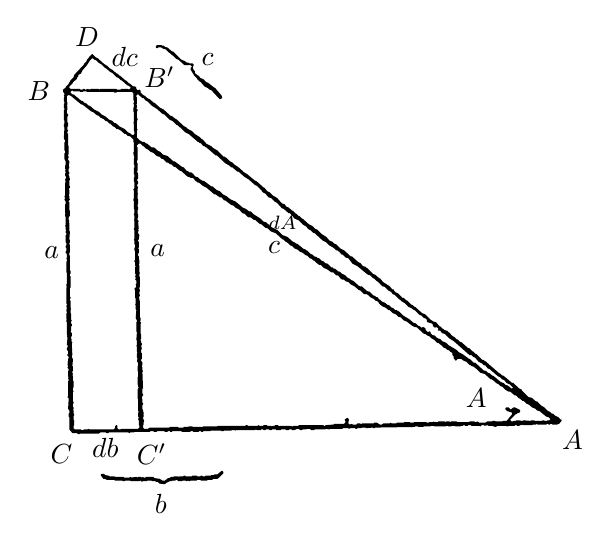
\begin{tikzpicture}[x=0.00773196cm,y=-0.00773196cm]
\fill[even odd rule] (343,754) -- (341,752) -- (340,752) -- (333,758) -- (328,758) -- (327,759) -- (323,759) -- (322,760) -- (314,760) -- (313,761) -- (309,761) -- (308,760) -- (306,760) -- (305,761) -- (300,761) -- (299,760) -- (292,760) -- (291,761) -- (281,761) -- (280,760) -- (278,760) -- (277,761) -- (271,761) -- (270,762) -- (268,761) -- (262,761) -- (261,762) -- (257,762) -- (254,764) -- (252,764) -- (247,768) -- (243,768) -- (238,765) -- (230,764) -- (228,762) -- (216,762) -- (215,763) -- (212,763) -- (211,762) -- (209,763) -- (207,762) -- (203,762) -- (202,763) -- (200,762) -- (192,763) -- (190,762) -- (189,763) -- (180,763) -- (179,762) -- (165,762) -- (164,761) -- (156,761) -- (155,760) -- (149,759) -- (147,757) -- (143,757) -- (142,758) -- (142,760) -- (146,765) -- (148,765) -- (152,767) -- (164,767) -- (165,768) -- (177,768) -- (178,769) -- (181,769) -- (182,768) -- (190,768) -- (191,769) -- (205,769) -- (207,768) -- (209,770) -- (211,769) -- (217,769) -- (218,768) -- (225,768) -- (226,769) -- (231,769) -- (232,770) -- (235,770) -- (238,773) -- (247,774) -- (249,772) -- (255,769) -- (258,769) -- (259,768) -- (264,768) -- (265,767) -- (267,767) -- (269,769) -- (275,769) -- (276,768) -- (281,768) -- (282,769) -- (285,768) -- (286,769) -- (288,769) -- (289,768) -- (299,768) -- (300,767) -- (305,767) -- (306,768) -- (316,768) -- (317,767) -- (324,767) -- (327,765) -- (333,765) -- (335,764) -- (343,756) -- cycle
(80,126) -- (80,130) -- (82,133) -- (82,135) -- (81,136) -- (82,138) -- (81,140) -- (81,145) -- (82,146) -- (82,149) -- (81,150) -- (81,156) -- (82,157) -- (82,159) -- (81,160) -- (81,176) -- (82,177) -- (82,182) -- (81,183) -- (81,187) -- (82,188) -- (81,206) -- (83,210) -- (83,212) -- (82,213) -- (82,226) -- (83,227) -- (83,230) -- (82,231) -- (82,240) -- (84,244) -- (84,250) -- (83,251) -- (83,256) -- (84,257) -- (83,260) -- (84,261) -- (84,263) -- (83,264) -- (83,267) -- (85,270) -- (83,274) -- (84,278) -- (83,279) -- (83,300) -- (82,301) -- (83,305) -- (82,307) -- (84,310) -- (84,314) -- (83,315) -- (83,328) -- (84,329) -- (83,331) -- (83,334) -- (84,335) -- (84,348) -- (83,350) -- (84,351) -- (84,356) -- (85,357) -- (84,359) -- (84,361) -- (85,362) -- (85,364) -- (84,365) -- (84,377) -- (85,378) -- (85,382) -- (84,383) -- (84,385) -- (85,386) -- (85,391) -- (84,392) -- (84,394) -- (86,396) -- (86,402) -- (85,403) -- (86,405) -- (86,408) -- (85,409) -- (85,426) -- (86,427) -- (86,445) -- (85,446) -- (85,449) -- (86,450) -- (85,452) -- (85,477) -- (86,478) -- (86,480) -- (85,481) -- (85,483) -- (86,484) -- (85,490) -- (86,491) -- (86,493) -- (85,494) -- (85,502) -- (86,504) -- (85,505) -- (85,507) -- (86,508) -- (86,528) -- (87,529) -- (86,531) -- (87,533) -- (86,545) -- (88,547) -- (86,551) -- (86,553) -- (88,556) -- (88,560) -- (87,561) -- (87,563) -- (89,565) -- (89,567) -- (88,568) -- (88,572) -- (87,573) -- (88,575) -- (87,577) -- (88,579) -- (87,583) -- (89,585) -- (89,587) -- (88,588) -- (88,597) -- (89,598) -- (88,600) -- (89,602) -- (89,604) -- (88,605) -- (88,629) -- (87,631) -- (89,633) -- (88,650) -- (90,653) -- (90,657) -- (89,658) -- (89,663) -- (90,664) -- (90,684) -- (95,690) -- (102,690) -- (106,692) -- (107,691) -- (138,691) -- (141,689) -- (150,689) -- (151,690) -- (154,690) -- (155,689) -- (187,689) -- (189,690) -- (190,689) -- (196,689) -- (197,688) -- (222,688) -- (223,687) -- (228,687) -- (229,688) -- (233,688) -- (234,687) -- (246,687) -- (247,688) -- (251,688) -- (252,687) -- (255,687) -- (256,688) -- (258,688) -- (259,687) -- (274,687) -- (275,688) -- (288,688) -- (289,687) -- (293,687) -- (294,688) -- (302,688) -- (303,687) -- (306,687) -- (307,688) -- (309,688) -- (310,687) -- (321,687) -- (322,686) -- (339,686) -- (340,687) -- (343,687) -- (344,686) -- (356,686) -- (357,685) -- (361,685) -- (363,686) -- (364,685) -- (395,685) -- (396,684) -- (398,685) -- (404,685) -- (405,684) -- (408,684) -- (409,685) -- (412,685) -- (413,684) -- (418,684) -- (419,685) -- (422,685) -- (423,684) -- (429,684) -- (430,685) -- (437,685) -- (438,684) -- (445,684) -- (446,685) -- (450,685) -- (451,684) -- (455,684) -- (456,685) -- (460,685) -- (464,683) -- (466,683) -- (469,685) -- (472,685) -- (473,684) -- (479,684) -- (480,683) -- (485,683) -- (487,685) -- (492,685) -- (493,684) -- (510,684) -- (511,683) -- (517,684) -- (518,683) -- (538,683) -- (539,682) -- (548,682) -- (549,683) -- (551,682) -- (559,682) -- (560,683) -- (562,683) -- (563,682) -- (569,682) -- (570,681) -- (576,681) -- (577,682) -- (588,681) -- (589,682) -- (591,682) -- (592,681) -- (657,680) -- (658,679) -- (662,679) -- (663,680) -- (671,680) -- (672,679) -- (683,679) -- (684,678) -- (688,678) -- (689,679) -- (708,679) -- (709,678) -- (711,678) -- (712,679) -- (717,679) -- (718,678) -- (723,678) -- (724,679) -- (732,679) -- (733,678) -- (736,678) -- (737,677) -- (739,677) -- (740,678) -- (744,678) -- (745,677) -- (749,677) -- (750,678) -- (763,678) -- (764,679) -- (765,679) -- (767,677) -- (771,677) -- (772,678) -- (777,677) -- (778,678) -- (785,678) -- (786,679) -- (790,680) -- (793,678) -- (807,678) -- (808,679) -- (810,679) -- (811,678) -- (821,678) -- (822,677) -- (824,677) -- (825,678) -- (829,678) -- (830,677) -- (833,677) -- (834,676) -- (836,677) -- (850,677) -- (851,676) -- (856,676) -- (857,675) -- (859,676) -- (873,676) -- (874,675) -- (876,675) -- (877,676) -- (879,676) -- (880,675) -- (882,675) -- (883,676) -- (891,676) -- (892,675) -- (894,675) -- (898,670) -- (898,668) -- (897,668) -- (893,664) -- (887,661) -- (884,658) -- (882,658) -- (879,655) -- (876,654) -- (870,648) -- (865,645) -- (858,638) -- (856,638) -- (849,632) -- (844,631) -- (833,620) -- (832,618) -- (830,618) -- (819,608) -- (816,607) -- (803,596) -- (800,595) -- (797,592) -- (796,592) -- (773,572) -- (772,572) -- (770,570) -- (768,570) -- (758,560) -- (757,560) -- (753,556) -- (752,556) -- (747,551) -- (744,550) -- (734,541) -- (731,540) -- (727,536) -- (726,536) -- (723,533) -- (718,530) -- (714,525) -- (713,525) -- (710,522) -- (706,521) -- (704,519) -- (703,519) -- (699,515) -- (698,515) -- (692,508) -- (688,507) -- (683,504) -- (674,495) -- (669,493) -- (658,483) -- (657,483) -- (654,480) -- (651,479) -- (644,472) -- (643,472) -- (639,468) -- (637,468) -- (630,461) -- (626,459) -- (623,456) -- (623,455) -- (622,454) -- (620,454) -- (616,449) -- (605,442) -- (600,436) -- (599,436) -- (592,430) -- (589,429) -- (579,419) -- (578,419) -- (576,417) -- (572,416) -- (568,411) -- (564,409) -- (554,400) -- (552,400) -- (541,390) -- (535,387) -- (528,380) -- (525,379) -- (522,376) -- (517,374) -- (512,368) -- (504,363) -- (497,356) -- (494,355) -- (489,350) -- (483,347) -- (473,338) -- (472,338) -- (468,334) -- (467,334) -- (463,330) -- (462,330) -- (457,325) -- (456,325) -- (449,319) -- (447,319) -- (443,314) -- (439,313) -- (431,304) -- (424,300) -- (419,295) -- (415,293) -- (410,287) -- (409,287) -- (398,277) -- (394,275) -- (382,265) -- (377,262) -- (367,253) -- (362,250) -- (358,246) -- (354,244) -- (348,238) -- (347,238) -- (345,236) -- (343,236) -- (333,226) -- (326,222) -- (323,219) -- (315,215) -- (309,208) -- (308,208) -- (304,204) -- (296,199) -- (291,194) -- (285,191) -- (282,188) -- (278,186) -- (265,174) -- (264,174) -- (259,170) -- (256,169) -- (245,159) -- (239,156) -- (230,148) -- (229,148) -- (222,142) -- (218,140) -- (215,137) -- (211,135) -- (207,131) -- (207,128) -- (205,126) -- (204,127) -- (202,127) -- (200,125) -- (200,123) -- (198,121) -- (195,121) -- (189,116) -- (188,116) -- (183,111) -- (182,111) -- (173,103) -- (172,103) -- (169,100) -- (168,100) -- (165,97) -- (164,97) -- (161,94) -- (156,91) -- (152,87) -- (147,84) -- (137,75) -- (133,73) -- (128,68) -- (127,68) -- (122,73) -- (122,74) -- (119,77) -- (118,80) -- (114,84) -- (114,85) -- (98,102) -- (97,106) -- (92,111) -- (88,118) -- (84,122) -- (84,123) -- cycle
(201,218) -- (204,215) -- (207,215) -- (211,219) -- (212,219) -- (216,223) -- (220,225) -- (223,228) -- (228,230) -- (232,234) -- (236,236) -- (238,236) -- (242,240) -- (244,240) -- (250,246) -- (252,246) -- (256,249) -- (258,249) -- (262,253) -- (264,253) -- (271,259) -- (274,260) -- (284,269) -- (288,270) -- (289,271) -- (293,271) -- (298,277) -- (299,277) -- (301,279) -- (303,279) -- (309,284) -- (315,287) -- (328,298) -- (330,298) -- (337,303) -- (340,303) -- (344,308) -- (346,308) -- (355,315) -- (360,317) -- (363,320) -- (369,323) -- (374,329) -- (378,330) -- (383,335) -- (385,336) -- (388,336) -- (393,340) -- (395,340) -- (403,347) -- (405,347) -- (412,353) -- (416,354) -- (421,359) -- (429,362) -- (440,372) -- (441,372) -- (444,375) -- (449,378) -- (453,382) -- (456,383) -- (460,387) -- (465,389) -- (468,392) -- (473,394) -- (478,398) -- (481,399) -- (485,403) -- (488,404) -- (491,407) -- (492,407) -- (497,412) -- (498,412) -- (500,414) -- (503,414) -- (508,419) -- (513,421) -- (520,426) -- (523,426) -- (528,431) -- (531,431) -- (536,437) -- (538,438) -- (541,438) -- (544,441) -- (548,442) -- (552,446) -- (558,449) -- (565,455) -- (568,456) -- (574,462) -- (578,462) -- (580,463) -- (584,467) -- (590,470) -- (593,473) -- (595,473) -- (598,476) -- (598,477) -- (604,482) -- (609,484) -- (614,488) -- (616,488) -- (621,493) -- (626,495) -- (630,499) -- (634,500) -- (639,505) -- (644,507) -- (653,514) -- (657,516) -- (660,516) -- (672,527) -- (674,527) -- (678,530) -- (681,531) -- (684,534) -- (689,537) -- (694,542) -- (696,542) -- (699,545) -- (700,545) -- (705,550) -- (708,551) -- (710,553) -- (713,554) -- (716,557) -- (717,557) -- (719,559) -- (719,562) -- (721,564) -- (721,567) -- (724,571) -- (725,571) -- (728,568) -- (733,568) -- (737,571) -- (742,573) -- (747,578) -- (748,578) -- (750,580) -- (754,581) -- (757,584) -- (758,584) -- (765,591) -- (772,593) -- (782,602) -- (784,602) -- (786,604) -- (787,604) -- (791,608) -- (795,610) -- (798,613) -- (801,614) -- (806,619) -- (811,622) -- (814,622) -- (821,628) -- (823,628) -- (828,633) -- (829,633) -- (834,637) -- (836,637) -- (841,642) -- (844,643) -- (850,648) -- (855,650) -- (858,653) -- (862,654) -- (873,663) -- (877,664) -- (880,667) -- (878,669) -- (875,669) -- (874,670) -- (870,670) -- (869,669) -- (867,669) -- (866,670) -- (854,670) -- (853,669) -- (848,669) -- (847,670) -- (835,669) -- (834,670) -- (831,670) -- (830,669) -- (824,669) -- (823,670) -- (819,670) -- (818,671) -- (816,671) -- (814,669) -- (814,668) -- (823,659) -- (824,659) -- (826,657) -- (828,657) -- (830,655) -- (830,652) -- (822,648) -- (819,648) -- (815,651) -- (814,651) -- (811,648) -- (807,648) -- (806,649) -- (806,651) -- (809,654) -- (816,656) -- (817,657) -- (817,659) -- (808,670) -- (802,670) -- (801,671) -- (790,671) -- (789,670) -- (785,670) -- (784,671) -- (776,671) -- (773,673) -- (763,673) -- (760,671) -- (758,672) -- (756,672) -- (755,671) -- (747,671) -- (746,672) -- (727,672) -- (726,671) -- (717,671) -- (716,672) -- (714,671) -- (709,671) -- (707,672) -- (706,671) -- (696,671) -- (695,672) -- (690,672) -- (688,671) -- (687,672) -- (681,672) -- (680,673) -- (677,673) -- (676,672) -- (656,672) -- (655,673) -- (650,673) -- (649,672) -- (640,672) -- (639,673) -- (628,673) -- (627,674) -- (619,674) -- (617,673) -- (616,674) -- (606,674) -- (603,676) -- (600,676) -- (595,673) -- (591,673) -- (590,674) -- (571,674) -- (570,675) -- (568,675) -- (567,674) -- (563,674) -- (561,676) -- (555,676) -- (554,675) -- (550,676) -- (548,674) -- (549,668) -- (548,666) -- (546,665) -- (542,668) -- (543,670) -- (543,673) -- (541,675) -- (525,675) -- (524,676) -- (511,677) -- (510,678) -- (508,678) -- (507,677) -- (467,677) -- (466,678) -- (458,678) -- (457,679) -- (455,679) -- (454,678) -- (437,678) -- (435,679) -- (432,677) -- (428,677) -- (427,678) -- (424,678) -- (422,679) -- (421,678) -- (415,678) -- (414,677) -- (409,677) -- (408,678) -- (402,678) -- (401,677) -- (399,678) -- (383,678) -- (382,677) -- (380,677) -- (379,678) -- (334,678) -- (333,679) -- (310,679) -- (309,680) -- (293,680) -- (292,679) -- (286,679) -- (285,680) -- (278,680) -- (277,681) -- (269,681) -- (268,680) -- (255,680) -- (254,681) -- (222,681) -- (219,683) -- (213,683) -- (211,681) -- (211,677) -- (212,676) -- (212,672) -- (213,670) -- (211,666) -- (211,664) -- (212,663) -- (212,656) -- (211,655) -- (211,652) -- (210,651) -- (210,644) -- (211,643) -- (211,641) -- (210,640) -- (210,634) -- (209,633) -- (210,629) -- (211,628) -- (211,626) -- (210,625) -- (210,617) -- (211,616) -- (210,590) -- (211,588) -- (210,587) -- (210,582) -- (209,581) -- (209,579) -- (210,578) -- (210,574) -- (208,572) -- (208,569) -- (209,568) -- (209,559) -- (208,558) -- (208,553) -- (209,552) -- (208,546) -- (209,545) -- (209,543) -- (208,542) -- (208,539) -- (207,538) -- (207,536) -- (208,535) -- (208,528) -- (207,527) -- (207,511) -- (208,509) -- (206,507) -- (207,505) -- (207,501) -- (206,500) -- (206,473) -- (205,472) -- (205,469) -- (204,468) -- (204,467) -- (206,465) -- (206,463) -- (205,462) -- (205,458) -- (206,457) -- (206,455) -- (205,454) -- (205,451) -- (206,450) -- (206,434) -- (205,433) -- (205,429) -- (206,427) -- (205,426) -- (205,415) -- (204,414) -- (205,412) -- (205,406) -- (204,405) -- (204,400) -- (203,399) -- (203,395) -- (204,394) -- (204,388) -- (203,387) -- (204,385) -- (204,376) -- (203,375) -- (203,373) -- (204,372) -- (205,365) -- (203,362) -- (203,359) -- (204,358) -- (203,356) -- (204,354) -- (203,344) -- (204,342) -- (202,340) -- (202,337) -- (203,336) -- (203,331) -- (202,330) -- (202,324) -- (203,323) -- (203,319) -- (202,318) -- (202,315) -- (203,314) -- (203,306) -- (202,305) -- (202,299) -- (203,297) -- (202,296) -- (202,289) -- (203,287) -- (201,283) -- (203,280) -- (203,278) -- (201,274) -- (203,272) -- (203,264) -- (201,261) -- (202,259) -- (202,247) -- (201,246) -- (201,243) -- (202,242) -- (202,221) -- (201,220) -- cycle
(88,135) -- (92,136) -- (109,150) -- (112,151) -- (126,162) -- (129,163) -- (135,168) -- (138,169) -- (141,172) -- (147,175) -- (150,178) -- (152,178) -- (156,182) -- (157,182) -- (161,186) -- (165,188) -- (168,191) -- (170,191) -- (174,193) -- (181,199) -- (183,199) -- (186,202) -- (190,203) -- (195,208) -- (195,212) -- (196,213) -- (196,228) -- (195,229) -- (195,232) -- (196,233) -- (196,236) -- (197,237) -- (196,239) -- (196,249) -- (197,250) -- (197,254) -- (196,255) -- (196,265) -- (197,266) -- (197,270) -- (196,271) -- (196,277) -- (197,278) -- (197,288) -- (195,290) -- (196,292) -- (196,305) -- (195,306) -- (195,308) -- (196,309) -- (196,322) -- (197,323) -- (197,329) -- (196,330) -- (196,332) -- (197,333) -- (197,339) -- (196,340) -- (197,342) -- (197,353) -- (196,354) -- (196,356) -- (197,357) -- (197,371) -- (196,373) -- (197,374) -- (197,380) -- (198,381) -- (198,385) -- (197,386) -- (197,390) -- (198,391) -- (198,406) -- (197,407) -- (197,409) -- (198,410) -- (198,415) -- (199,416) -- (198,418) -- (198,428) -- (199,429) -- (199,431) -- (198,432) -- (199,436) -- (198,438) -- (200,440) -- (200,445) -- (199,446) -- (200,450) -- (197,453) -- (197,454) -- (198,455) -- (198,468) -- (199,469) -- (199,477) -- (198,479) -- (199,480) -- (199,487) -- (200,488) -- (199,501) -- (201,505) -- (201,507) -- (200,508) -- (200,523) -- (201,524) -- (200,537) -- (201,538) -- (201,545) -- (200,547) -- (201,548) -- (201,557) -- (202,558) -- (201,560) -- (201,566) -- (202,567) -- (201,572) -- (203,575) -- (203,579) -- (202,580) -- (202,588) -- (203,589) -- (203,597) -- (202,598) -- (202,610) -- (203,611) -- (203,614) -- (204,615) -- (202,619) -- (202,633) -- (203,634) -- (203,654) -- (204,655) -- (203,657) -- (203,663) -- (204,664) -- (203,668) -- (204,669) -- (204,677) -- (205,678) -- (205,681) -- (203,683) -- (175,683) -- (174,684) -- (171,684) -- (169,682) -- (169,678) -- (168,677) -- (167,677) -- (165,679) -- (165,682) -- (163,684) -- (123,684) -- (121,683) -- (120,684) -- (114,684) -- (113,685) -- (110,685) -- (109,684) -- (99,684) -- (97,682) -- (97,678) -- (98,677) -- (98,669) -- (97,668) -- (97,662) -- (98,661) -- (98,659) -- (97,658) -- (97,653) -- (96,652) -- (97,650) -- (97,648) -- (96,647) -- (96,642) -- (97,641) -- (97,639) -- (96,638) -- (96,623) -- (97,622) -- (96,620) -- (96,616) -- (97,615) -- (97,605) -- (96,604) -- (96,596) -- (95,595) -- (96,593) -- (95,591) -- (95,589) -- (96,588) -- (96,581) -- (95,580) -- (96,569) -- (94,565) -- (94,563) -- (95,562) -- (94,543) -- (95,541) -- (93,539) -- (94,537) -- (93,535) -- (93,532) -- (94,531) -- (94,526) -- (92,523) -- (93,521) -- (93,515) -- (94,514) -- (94,511) -- (93,510) -- (93,507) -- (94,505) -- (93,504) -- (93,494) -- (92,493) -- (92,488) -- (93,486) -- (92,485) -- (92,473) -- (91,472) -- (91,470) -- (92,469) -- (92,467) -- (91,466) -- (91,452) -- (92,451) -- (92,433) -- (91,432) -- (91,429) -- (92,428) -- (92,424) -- (91,423) -- (91,399) -- (90,398) -- (90,394) -- (91,393) -- (91,381) -- (90,380) -- (90,378) -- (91,377) -- (91,373) -- (90,372) -- (91,359) -- (90,358) -- (90,345) -- (89,344) -- (90,342) -- (89,340) -- (89,336) -- (91,333) -- (91,325) -- (90,324) -- (90,311) -- (89,310) -- (89,309) -- (91,307) -- (90,305) -- (90,301) -- (89,300) -- (90,298) -- (90,291) -- (89,289) -- (91,287) -- (91,285) -- (90,284) -- (90,275) -- (91,274) -- (91,272) -- (90,271) -- (90,268) -- (89,267) -- (89,265) -- (90,264) -- (90,262) -- (89,261) -- (89,256) -- (90,255) -- (89,248) -- (90,247) -- (90,244) -- (88,241) -- (88,239) -- (89,238) -- (89,236) -- (88,235) -- (88,233) -- (89,232) -- (89,219) -- (88,218) -- (88,199) -- (87,198) -- (87,195) -- (88,194) -- (87,192) -- (87,187) -- (88,186) -- (88,181) -- (87,180) -- (87,170) -- (88,169) -- (88,167) -- (86,165) -- (86,160) -- (87,159) -- (87,154) -- (86,153) -- (87,151) -- (87,147) -- (86,146) -- (86,137) -- cycle
(200,136) -- (202,134) -- (203,134) -- (210,140) -- (212,140) -- (215,144) -- (219,146) -- (226,153) -- (234,158) -- (243,166) -- (246,167) -- (254,175) -- (260,178) -- (266,184) -- (267,184) -- (271,188) -- (272,188) -- (280,196) -- (286,199) -- (301,212) -- (302,212) -- (304,214) -- (306,214) -- (310,219) -- (312,219) -- (314,221) -- (315,221) -- (330,234) -- (332,234) -- (346,247) -- (353,251) -- (356,254) -- (358,254) -- (366,261) -- (368,261) -- (377,269) -- (385,274) -- (395,283) -- (398,284) -- (406,292) -- (406,293) -- (408,295) -- (412,297) -- (417,303) -- (421,304) -- (427,310) -- (431,312) -- (439,321) -- (442,322) -- (450,329) -- (452,329) -- (460,338) -- (467,341) -- (474,348) -- (479,351) -- (482,355) -- (486,357) -- (490,361) -- (493,362) -- (506,374) -- (512,377) -- (517,382) -- (524,386) -- (528,390) -- (530,390) -- (532,392) -- (533,392) -- (537,397) -- (539,397) -- (544,402) -- (548,403) -- (555,412) -- (563,416) -- (580,430) -- (584,431) -- (589,436) -- (590,436) -- (595,441) -- (596,441) -- (604,449) -- (608,450) -- (614,456) -- (618,458) -- (621,462) -- (624,463) -- (632,471) -- (633,471) -- (636,474) -- (641,477) -- (647,483) -- (652,485) -- (654,487) -- (658,489) -- (665,496) -- (668,497) -- (672,501) -- (675,502) -- (677,504) -- (677,507) -- (678,508) -- (685,510) -- (687,512) -- (687,515) -- (688,515) -- (690,517) -- (693,516) -- (696,519) -- (695,521) -- (696,522) -- (699,522) -- (702,526) -- (706,527) -- (713,534) -- (721,539) -- (747,562) -- (750,562) -- (753,565) -- (756,566) -- (762,573) -- (768,576) -- (771,579) -- (773,579) -- (777,584) -- (780,585) -- (794,597) -- (797,598) -- (801,602) -- (804,603) -- (808,608) -- (813,610) -- (818,615) -- (818,616) -- (816,617) -- (810,612) -- (806,611) -- (803,608) -- (798,606) -- (786,596) -- (785,596) -- (780,592) -- (777,591) -- (774,588) -- (770,587) -- (757,575) -- (753,574) -- (747,568) -- (746,568) -- (735,560) -- (729,557) -- (725,553) -- (713,546) -- (709,542) -- (702,539) -- (699,536) -- (694,534) -- (690,530) -- (686,529) -- (683,526) -- (683,524) -- (681,523) -- (680,524) -- (678,524) -- (675,521) -- (675,519) -- (673,517) -- (671,516) -- (668,517) -- (666,515) -- (663,514) -- (659,510) -- (655,509) -- (648,503) -- (638,497) -- (632,491) -- (627,488) -- (625,488) -- (622,485) -- (619,484) -- (615,480) -- (613,480) -- (608,476) -- (603,474) -- (600,471) -- (599,471) -- (596,467) -- (594,467) -- (592,465) -- (589,464) -- (583,458) -- (579,457) -- (570,449) -- (567,449) -- (565,448) -- (556,440) -- (553,439) -- (551,437) -- (547,435) -- (543,431) -- (537,428) -- (534,425) -- (532,425) -- (526,420) -- (524,420) -- (522,418) -- (520,418) -- (514,412) -- (510,411) -- (507,408) -- (504,407) -- (500,403) -- (498,403) -- (496,401) -- (492,400) -- (489,397) -- (486,396) -- (480,390) -- (479,390) -- (477,388) -- (475,388) -- (464,379) -- (462,379) -- (460,377) -- (457,376) -- (448,368) -- (440,365) -- (432,357) -- (422,352) -- (413,344) -- (409,343) -- (404,338) -- (393,331) -- (388,326) -- (385,326) -- (380,322) -- (375,320) -- (363,310) -- (354,306) -- (348,301) -- (342,298) -- (337,293) -- (332,291) -- (325,285) -- (323,285) -- (311,276) -- (309,276) -- (304,273) -- (301,270) -- (297,269) -- (294,266) -- (294,265) -- (290,262) -- (287,262) -- (285,260) -- (283,260) -- (278,254) -- (275,253) -- (263,244) -- (261,244) -- (251,235) -- (244,233) -- (239,228) -- (236,227) -- (229,221) -- (225,221) -- (218,215) -- (215,214) -- (213,212) -- (210,212) -- (205,209) -- (201,205) -- (201,193) -- (202,192) -- (201,190) -- (201,177) -- (202,176) -- (202,174) -- (201,173) -- (201,162) -- (202,161) -- (202,159) -- (200,157) -- (201,155) -- (201,152) -- (200,151) -- (201,149) -- (201,139) -- (200,138) -- cycle
(92,130) -- (94,128) -- (96,128) -- (97,129) -- (107,129) -- (108,130) -- (112,130) -- (113,129) -- (118,129) -- (119,130) -- (163,130) -- (164,131) -- (167,131) -- (168,130) -- (193,130) -- (195,132) -- (195,143) -- (196,144) -- (196,148) -- (195,149) -- (196,151) -- (196,155) -- (195,156) -- (195,162) -- (196,163) -- (196,179) -- (195,181) -- (196,182) -- (196,194) -- (197,195) -- (197,199) -- (195,201) -- (192,200) -- (190,198) -- (186,196) -- (181,191) -- (173,187) -- (166,181) -- (164,181) -- (160,177) -- (156,176) -- (149,170) -- (143,167) -- (139,163) -- (131,159) -- (124,153) -- (121,152) -- (118,149) -- (115,148) -- (112,145) -- (109,144) -- (97,134) -- (95,134) -- (92,131) -- cycle
(90,121) -- (96,115) -- (96,114) -- (102,109) -- (103,106) -- (105,104) -- (105,102) -- (109,100) -- (112,94) -- (119,86) -- (124,78) -- (127,75) -- (129,75) -- (131,77) -- (134,78) -- (138,82) -- (143,85) -- (149,91) -- (150,91) -- (157,97) -- (161,99) -- (168,106) -- (171,107) -- (175,111) -- (176,111) -- (185,119) -- (188,120) -- (191,123) -- (188,126) -- (186,125) -- (175,125) -- (174,126) -- (168,126) -- (167,125) -- (141,125) -- (140,126) -- (138,125) -- (125,125) -- (124,126) -- (119,125) -- (118,126) -- (116,126) -- (115,125) -- (113,125) -- (112,126) -- (108,126) -- (107,125) -- (92,125) -- (90,123) -- cycle
(232,55) -- (232,57) -- (233,58) -- (235,58) -- (236,57) -- (241,57) -- (244,59) -- (248,60) -- (254,66) -- (255,66) -- (259,70) -- (260,70) -- (266,76) -- (269,77) -- (279,86) -- (289,86) -- (291,88) -- (291,89) -- (289,91) -- (289,93) -- (295,103) -- (300,108) -- (300,109) -- (304,113) -- (305,113) -- (312,121) -- (318,124) -- (320,126) -- (323,127) -- (337,142) -- (341,140) -- (340,136) -- (329,123) -- (328,123) -- (318,115) -- (315,114) -- (310,109) -- (305,107) -- (302,103) -- (301,103) -- (296,99) -- (296,96) -- (293,92) -- (293,88) -- (294,87) -- (294,85) -- (292,83) -- (287,83) -- (286,82) -- (283,82) -- (279,79) -- (274,77) -- (261,64) -- (258,63) -- (251,57) -- (247,56) -- (245,54) -- (242,54) -- (241,53) -- (234,53) -- cycle;
\node[inner sep=0pt,font=\fontsize{10}{12}\selectfont] at (119,40) {$D$};
\node[inner sep=0pt,font=\fontsize{10}{12}\selectfont] at (181,73) {$dc$};
\node[inner sep=0pt,font=\fontsize{10}{12}\selectfont] at (238,106) {$B'$};
\node[inner sep=0pt,font=\fontsize{10}{12}\selectfont] at (317,77) {$c$};
\node[inner sep=0pt,font=\fontsize{10}{12}\selectfont] at (40,128) {$B$};
\node[inner sep=0pt,font=\fontsize{10}{12}\selectfont] at (61,394) {$a$};
\node[inner sep=0pt,font=\fontsize{10}{12}\selectfont] at (235,390) {$a$};
\node[inner sep=0pt,font=\fontsize{10}{12}\selectfont] at (426,386) {$c$};
\node[inner sep=0pt,font=\fontsize{7}{9}\selectfont] at (440,344) {$dA$};
\node[inner sep=0pt,font=\fontsize{10}{12}\selectfont] at (758,632) {$A$};
\node[inner sep=0pt,font=\fontsize{10}{12}\selectfont] at (77,724) {$C$};
\node[inner sep=0pt,font=\fontsize{10}{12}\selectfont] at (149,714) {$db$};
\node[inner sep=0pt,font=\fontsize{10}{12}\selectfont] at (225,725) {$C'$};
\node[inner sep=0pt,font=\fontsize{10}{12}\selectfont] at (240,806) {$b$};
\node[inner sep=0pt,font=\fontsize{10}{12}\selectfont] at (916,701) {$A$};
\end{tikzpicture}


Fig. 7.
\end{minipage}\end{center}
